%%-------------------------Data generation---------------------------------------%%

There are no practically useful parametric models available, for our knowledge only models available so far, \cite{stein1999} with 170 parameters to estimate and \cite{CressieJohannesson2008} more than 396 parameters to estimate. The previous studies have argued that many processes on a sphere are not homogeneous, especially in the direction of latitude. \cite{JunStein2008} proposed flexible class of parametric covariance models to capture the non-stationarity of global data. They used Discrete Fourier Transform (DFT) to the data on regular grids and calculated the exact likelihood for large data sets. Furthermore, they used Legendre polynomials to remove the spatial trends when fitting models to global data.  
\cite{Huang2012} proposed a class of statistical processes that are axially symmetric and covariance functions that depend on longitudinal differences. Moreover, they have proposed longitudinally reversible processes and some motivations to construct axially symmetric processes.

Li \cite{Li2013} discussed about the issues associated when modeling axially symmetric spatial random fields on a sphere. Further, They proposed convolution methods to generate random fields with a class of $Mat\acute{e}rn$-type kernel functions by allowing the parameters in the kernel function to vary with location. Moreover, they were able to generate flexible class of covariance functions and capture the non-stationary properties on a sphere. Monte Carlo Markov Chain (MCMC) is another approach to model non-stationary covariance models on a sphere. \cite{BolinLindgren2011} (continuation of the work proposed in \cite{Lindgren2011} ) constructed a class of stochastic field models using Stochastic Partial Differential Equations (SPDEs). Non stationary covariance models were obtained by spatially varying the parameters in the SPDEs, they argue that this method is more efficient than standard MCMC procedures. 

\cite{HitczenkoStein2012} discuss about the properties of an existing class of models for axially symmetric Gaussian processes on the sphere. They applied first-order differential operators to an isotropic process. draw conclusions about the local properties of the processes. Under some restrictions they derived explicit forms for the spherical harmonic representation of these processes covariance functions, and make conclusions about the local properties of the processes.

$Mat\acute{e}rn$ covariance models are widely used when modeling spatial data, but when the smoothness parameter ($\nu$) is greater than 0.5 it is not valid for the homogeneous processes on the Earth surface with great circle distance. \cite{JeongJun2015} proposed $Mat\acute{e}rn$-like covariance functions for smooth processes on the earth surface that are valid with great circle distance (models were tested on sea levels pressure data).


The global data generation process on a sphere discussed on this dissertation is primarily based on the axially symmetric covariance structure introduced by \cite{Jones1963} and as continuation of axially symmetric process on a sphere developed by \cite{Huang2012}.  Let $X(P)$ be a complex-valued random process defined on a unit sphere $S^2$, where $P = (\lambda, \phi) \in S^2$ with longitude $\lambda \in [-\pi, \pi)$ and latitude $\phi \in [0, \pi]$. In chapter 4 we discussed how to formulate a valid covariance function for continuous axially symmetric processes on a sphere and was given by \ref{R(PQ)-01}. Now, in the light of \cite{Huang2012}[remark 2.5] a continuous axially symmetric process, $X(P)$ on a unit sphere , is given by
			
	\beq \label{process_sphere}
	X(P) = X(\phi, \lambda) = \sum_{m=-\infty}^{\infty} W_{m, \nu}(\phi) e^{i m \lambda}\psi_{m,\nu} (\phi),
	\eeq
			
	where $\lambda$ is the longitude, $\phi$ is the latitude and $\psi_{m,\nu}(\cdot)$ is a orthonormal basis for \Cm and using inverse Fourier transformation we get
	\[
		W_m(\phi) = \frac{1}{2\pi} \int_{S^2} X(P) e^{-im\lambda} \overline{\psi_{m,\nu} (\phi)} dP,
	\]
	with $\mbox{E}(W_{m, \nu} \overline{W_{n,\nu}}) = \delta_{m,n}\delta_{m,\mu}\eta_{m,\nu}$. \\
			
	{\bf Remark 1} If the random process on a sphere is real-Gaussian, then the weights given by $W_{m,\nu}$ will be independent normal random variables. Furthermore, if $\nu$ is fixed the process defined by $X(P)$ will be equivalent to a homogeneous random process on a circle with angular distance $\Delta \lambda$. In other words a random process on a sphere at a given latitude (for fix $\phi$) can be studies as a random process on the circle. In Chapter 3 \label{process_circle} a random process on a circle was given by a infinite Fourier summation (\cite{Roy1972},\cite{DUFOUR1976107}) and in the case of a process on a circle, $X(P)$ (\ref{process_sphere}) can be given by   
			
	\beq \label{eq:sym_process} 
	X(\phi, \lambda) = \sum_{m=-\infty}^{\infty} W_m(\phi) e^{i m \lambda},
	\eeq
			
	\[
		\mbox{where } W_m(\phi) = \frac{1}{2\pi} \int_0^{2\pi} X(\phi, \lambda) e^{-i m \lambda} d \lambda,
	\]
			
	with $\mbox{E}(W_m(\phi_P) \overline{W_n(\phi_Q)}) = \delta_{m,n} C_m(\phi_P, \phi_Q)$. \\
		
	%-------------------------------------% 
	\subsection{Deriving \Cm}
	%-------------------------------------%	
	%%%%%%%% this is the Appendix A n in data generation paper
%%%%%%%% details of deriving C_m

%\documentclass[12pt, amstex, letterpaper] {report} %{article}


\usepackage[margin=1in]{geometry}
\topmargin -0.5in \textwidth 6.5in \textheight 9in
\footskip .5in
\headheight 0.3in


\usepackage{Sweave}

\DefineVerbatimEnvironment{Sinput}{Verbatim} {xleftmargin=0em,frame=single}
\DefineVerbatimEnvironment{Soutput}{Verbatim} {xleftmargin=0em,frame=single}

\usepackage{amssymb, mathrsfs, amsmath, amsfonts}
\usepackage{enumerate, comment}
\usepackage{hyperref, natbib,apalike, float} %cite
\usepackage{color, multirow, setspace, fancyhdr,graphicx}
\usepackage{undertilde}
\usepackage[bottom]{footmisc}
\usepackage{graphicx}
\usepackage{framed}
\usepackage{subcaption}
\usepackage{amsthm}

%\doublespacing
\pagestyle{empty}
\pagestyle{fancy}
\lhead{ }
%\rhead{May 2016}
\fancyfoot{ }
\rfoot{Dissertation $|$ \thepage}
\lfoot{Chris Vanlangenberg}
\date{}

\includecomment{comment}

\newtheorem{theorem}{Theorem}[section]
\newtheorem{defn}{Definition}[section]
\newtheorem{prop}{Proposition}
\newcommand{\pro}[1]{\begin{prop}{#1}\end{prop}}

%\newtheorem{proof}{proof}
\newtheorem{rmk}{Remark}
\newcommand{\rmark}[1]{\begin{rmk}{#1}\end{rmk}}

\numberwithin{equation}{section}
\renewcommand{\footrulewidth}{0.1pt}
\renewcommand{\headrulewidth}{0.1pt}


\newcommand{\eqn}[1]{\begin{equation}{#1}\end{equation}}

\newcommand{\beq}{\begin{equation}}
\newcommand{\eeq}{\end{equation}}
%\renewcommand\refname{Literature}
\newcommand{\blue}[1]{\textcolor{blue}{\emph{#1}}}
\newcommand{\red}[1]{\textcolor{red}{\emph{#1}}}
\newcommand{\twoc}[2]{{\textcolor{blue}{#1}} and {\textcolor{red}{#2}}}


\newcommand{\xn}{x_1,\ldots, x_n}
\newcommand{\Xn}{X_1,\ldots, X_n}
\newcommand\floor[1]{\lfloor{#1}\rfloor}
\newcommand\ceil[1]{\lceil{#1}\rceil}

\newcommand{\X}{\mathcal{X}}
\newcommand{\Sp}{\mathbb{S}}
\newcommand{\R}{\mathbb{R}}
\newcommand{\C}{\mathbb{C}}
\newcommand{\pd}{positive definite }



\newcommand{\code}[1]{{\small\texttt{#1}}}
\newcommand{\pkg}[1]{{\normalfont\textsf{#1}}}
\newcommand{\var}[1] {{\normalfont\textbf{#1}}}
\newcommand{\Cm}{$C_m(\phi_P, \phi_Q)\ $}

\newcommand{\jun}{\cite{JunStein2008}}
%\begin{document}

In general for covariance function defined on a sphere (\cite{Stein2007}) requires triple summation and required to estimate $\mathcal{O}(n^3)$ parameters. In contrast, the covariance function  defined by \cite{Huang2012} requires to estimate $\mathcal{O}(n^2)$ parameters which is a huge reduction of computational complexity. We continued to use this covariance models discussed on chapter 4 in our approach on global data generation. In our approach it is very crucial to derive \Cm based on a known $R(P,Q)$, the detailed steps to derive \Cm for model1 (\ref{model1}) is given below,

%% C_m(P,Q) 
%% C_1\left(C_2 - e^{-a|\phi_P|} - e^{-a|\phi_Q|} + e^{-a|\phi_P - \phi_Q|}\right)

\begin{eqnarray*}
	R(P, Q) &=& R(\phi_P, \phi_Q, \Delta \lambda) = \tilde{C}(\phi_P, \phi_Q) \frac{1-p^2}{1 - 2p \cos(\Theta)+p^2},
\end{eqnarray*}

where $\Theta = \Delta \lambda + u(\phi_P - \phi_Q),$ with some choice of $C_1, C_2, a, u,$ and $p$.

Now,

\begin{eqnarray*}
	C_m(\phi_P, \phi_Q) &=& \frac{1}{2\pi} \int_{-\pi}^\pi R(\phi_P, \phi_Q, \Delta \lambda) e^{-im\Delta \lambda}d\Delta \lambda \\
	&=& \tilde{C}(\phi_P, \phi_Q) \frac{1}{2\pi}\int_{-\pi}^\pi \frac{1-p^2}{1 - 2p \cos(\Theta+p^2} e^{-im\Delta \lambda}d\Delta \lambda
\end{eqnarray*}

Next we focus on the following integration.

\begin{eqnarray*}
	\int_{-\pi}^\pi \frac{1-p^2}{1 - 2p \cos(x+b)+p^2} e^{-imx}dx ,
\end{eqnarray*}

where we set $x=\Delta\lambda$ and $b=u(\phi_P -\phi_Q)$ and we have,

\begin{eqnarray*}
	\frac{1-p^2}{1 - 2p \cos(x+b)+p^2} &=& \frac{2-2p\cos(x+b)-(1-2p \cos(x+b)+p^2)}{1-2p \cos(x+b)+p^2}\\
	&=& 2\times \frac{1-p\cos(x+b)}{1-2p \cos(x+b)+p^2}-1 \\
	&=& 2\times \sum_{n=0}^{\infty}p^n\cos n(x+b)-1  \\
	&=& 1 + 2 \sum_{n=1}^{\infty}p^n (\cos nx \cos(nb) - \sin(nx) \sin(nb)).
\end{eqnarray*}
Therefore, for $m \ne 0$,
\begin{eqnarray*}
	& & \int_{-\pi}^\pi \frac{1-p^2}{1 - 2p \cos(x+b)+p^2} e^{-imx}dx \\
	&=& \int_{-\pi}^\pi \left[1 + 2 \sum_{n=1}^{\infty}p^n (\cos nx \cos(nb) - \sin(nx) \sin(nb))\right]  e^{-imx}dx \\
	&=& \int_{-\pi}^\pi e^{-imx}dx + 2 \sum_{n=1}^{\infty}p^n \int_{-\pi}^\pi \left[\cos nx \cos(nb) - \sin(nx) \sin(nb)\right]  e^{-imx}dx \\
	&=& 2 \sum_{n=1}^{\infty}p^n \left[\cos(nb)  \int_{-\pi}^\pi \cos(nx) e^{-imx} dx - \sin(nb)  \int_{-\pi}^\pi \sin(nx) e^{-imx}dx \right] \\
	&=& 2 \sum_{n=1}^{\infty}p^n \left[ \pi \cos(nb) \delta(n, m) + \pi i\sin(nb)\right] \\
	&=& 2\pi p^m e^{imb}
\end{eqnarray*}
That is, for $m \ne 0$,

\begin{eqnarray*}
	C_m(\phi_P, \phi_Q)  &=& \tilde{C}(\phi_P, \phi_Q) \frac{1}{2\pi} (2\pi p^m e^{imb}) \\
	&=& \tilde{C}(\phi_P, \phi_Q) p^m e^{imb}.
\end{eqnarray*}
And for $m = 0$, $C_0(\phi_P, \phi_Q) = \tilde{C}(\phi_P, \phi_Q)$.\\

In summary,

\begin{eqnarray*}
	C_m(\phi_P, \phi_Q) &=& \left\{ \begin{array}{ll}
	\tilde{C}(\phi_P, \phi_Q), & m = 0 \\
	\tilde{C}(\phi_P, \phi_Q)p^m e^{imb}, & m \ne 0.
	\end{array}
	\right.\\
	%&=& C_1\left(C_2 - e^{-a|\phi_P|} - e^{-a|\phi_Q|} + e^{-a|\phi_P - \phi_Q|}\right)p^m (\cos(mu(\phi_P - \phi_Q))+i \sin(mu(\phi_P - \phi_Q))).
\end{eqnarray*}

If the process is longitudinally reversible one can set $u=0$ suppose $\tilde{C}(\phi_P, \phi_Q)$ given by \ref{Cm_model1} then \Cm for model1,

\begin{eqnarray*}
	C_m(\phi_P, \phi_Q) &=& \left\{ \begin{array}{ll}
	C_1\left(C_2 - e^{-a|\phi_P|} - e^{-a|\phi_Q|} + e^{-a|\phi_P - \phi_Q|}\right)  & m = 0 \\
	C_1\left(C_2 - e^{-a|\phi_P|} - e^{-a|\phi_Q|} + e^{-a|\phi_P - \phi_Q|}\right)p^m & m \ne 0.
	\end{array}
	\right.
\end{eqnarray*}


%\end{document}
	
			
		
	%%------------------------------------------------------------------%% 
	\section{Method development}
	%%------------------------------------------------------------------%%
			
			
	We can construct normal independent (complex) random variate $W_m(\phi)$ associated with the variance-covariance matrix $C_m(\phi_P, \phi_Q)$ to construct an axially symmetric process for a given latitude $\phi$. Then finite summation can be used to approximate above (\ref{eq:sym_process}) infinite summation as given below,
	\beq
	X(P) = X(\phi, \lambda) = \sum_{m=-N}^{N} W_m(\phi) e^{i m \lambda}
	\eeq
	where this would provide  the gridded data.
	Since $W_m$'s are independent for $m = 1, 2, \cdots$, we have
			
	\begin{eqnarray*}
		Cov(X(P), {X(Q)}) &=& Cov\left(\sum_{m = -N}^{N} W_m(\phi_P) e^{i m \lambda_P}, \sum_{j=-N}^{N} {W_j(\phi_Q)} e^{i j \lambda_Q}\right) \\
		&=& \sum_{m, j} e^{i m \lambda_P} e^{-i j \lambda_Q} Cov(W_m(\phi_P), {W_j(\phi_Q)}) \\
		&=& \sum_{m} e^{im (\lambda_P - \lambda_Q)} C_m(\phi_P, \phi_Q)
	\end{eqnarray*}
			
	The above generated data will be complex random variates. Therefore to have the real-valued data observations or to obtain a real process, we need to have
	\beq \label{eq:for_real}
	C_{-m} (\phi_P, \phi_Q) = \overline{C_m(\phi_P, \phi_Q)}, \quad \mbox{for $m = 1, 2, \cdots, N$}
	\eeq
	Lets write $W_m(\phi) = W_{m}^{r}(\phi) + i W_{m}^i(\phi)$ in terms of a real component and an imaginary component. We also write $C_m(\phi_P, \phi_Q) = C_m^r(\phi_P, \phi_Q) + i C_m^i(\phi_P, \phi_Q)$
	and with the relationship \ref{eq:for_real} above, we have
	\[
		C_{-m}^r(\phi_P, \phi_Q) = C_{-m}^r(\phi_P, \phi_Q), \quad C_{-m}^i(\phi_P, \phi_Q) = - C_{-m}^i(\phi_P, \phi_Q).
	\]
	Now,
	\begin{eqnarray*}
		Cov(W_m(\phi_P), {W_m(\phi_Q)}) &=& Cov(W_m^r(\phi_P) + iW_m^i(\phi_P), W_m^r(\phi_Q) + i W_m^i(\phi_Q)) \\
		&=& \left[Cov(W_m^r(\phi_P), W_m^r(\phi_Q)) + Cov(W_m^i(\phi_P), W_m^i(\phi_Q))\right] \\
		& & + i\left[- Cov(W_m^r(\phi_P), W_m^i(\phi_Q)) + Cov(W_m^i(\phi_P), W_m^r(\phi_Q))\right] \\
		&=& C_m^r(\phi_P, \phi_Q) + i C_m^i(\phi_P, \phi_Q).
	\end{eqnarray*}
	If we let $W_{-m}(\phi) = \overline{W_m(\phi)}$, then the covariance function would satisfy the above relationship \ref{eq:for_real}. In addition, we will set the following,
			
	\begin{eqnarray} \label{real_cov}
		& & Cov(W_m^r(\phi_P), W_m^r(\phi_Q)) = Cov(W_m^i(\phi_P), W_m^i(\phi_Q)) = \frac{1}{2}C_m^r(\phi_P, \phi_Q) \label{real_cov},
	\end{eqnarray}
	\begin{eqnarray} \label{im_cov}
		& & Cov(W_m^i(\phi_P), W_m^r(\phi_Q)) = - Cov(W_m^r(\phi_P), W_m^i(\phi_Q)) = \frac{1}{2}C_m^i(\phi_P, \phi_Q).
	\end{eqnarray}
			
	Therefore, if we denote $\utilde{W}_m(\phi) = (W_m^r(\phi), W_m^i(\phi))^T$, then the variance-covariance matrix for $\utilde{W}_m(\phi)$ is given by
			
	\[
		\frac{1}{2}\left(\begin{array}{ll}
		C_m^r(\phi_P, \phi_Q)& -C_m^i(\phi_P, \phi_Q) \\
		C_m^i(\phi_P, \phi_Q) & C_m^r(\phi_P, \phi_Q)
		\end{array}
		\right).
	\]
			
	However, we cannot have a vector of random variables $\utilde{W}_m(\phi)$ with a non-symmetric variance-covariance matrix unless $C_m^i(\phi_P, \phi_Q) = 0$. In the next section we will demonstrate how to generate $\utilde{W}_m(\phi)$ with a symmetric variance-covariance\\
			
	The process given by (\ref{eq:sym_process}) is now simplified as the following (real) process,
			
	\begin{eqnarray} \label{eq:finite_process}
		X(P) &=& \sum_{m = -N}^N W_m(\phi) e^{im \lambda} =  W_0(\phi) + \sum_{m =1}^N W_m(\phi) e^{im \lambda} + \sum_{m =-1}^{-N} W_m(\phi) e^{im \lambda} \nonumber \\
		&=& W_0(\phi) + \sum_{m =1}^N W_m(\phi) e^{im \lambda} + \sum_{m =1}^{N} \overline{W_m(\phi)} e^{-im \lambda} \nonumber \\
		&=& W_0(\phi) + \sum_{m =1}^N \left[  (W_m^r(\phi)+iW_m^i(\phi))(\cos(m \lambda) + i \sin(m \lambda)) \right. \nonumber \\
		& & \left. +\ (W_m^r(\phi)-iW_m^i(\phi))(\cos(m \lambda) - i \sin(m \lambda))  \right]  \nonumber \\
		&=& W_0(\phi) + 2 \sum_{m =1}^N \left[W_m^r(\phi)\cos(m\lambda) - W_m^i(\phi)\sin(m \lambda)\right].
	\end{eqnarray}
			
			
			
	%-------------------------------------% 
	\subsection{Data generation}
	%-------------------------------------% 
			
	Now for each fixed $m = 0, 1, 2, \cdots, N$, we consider  $W_m(\phi) = W_m^r(\phi) + i W_m^i(\phi)$ then $W_m^*(\phi) = W_m^r(\phi) - i W_m^i(\phi)$ (where $W_m^*(\phi)$ is the complex conjugate of $W_m(\phi)$). We may assume that $W_m^r(\phi)$ and $W_m^i(\phi)$ are independent, each following a (Gaussian) distribution with mean zero and the same variance $\sigma_m^2(\phi) = \frac{1}{2}C_m^r(\phi, \phi)$, ($C_m^i(\phi, \phi) = 0$ implies $W_m^r(\phi)$ and $W_m^i(\phi)$ are uncorrelated, or independent for Gaussian). In chapter 1 we introduced the concept of circularly-symmetry, thus according to \cite{Gallager2008} a complex random variable is circularly-symmetric if and only if it pseudo covariance is zero (\ref{circular_theory}). In this section we will show that the Gaussian random variable $W_m(\phi)$ is a circularly-symmetric complex random variable.  \\
			
	Now for a set of distinct latitudes $\Phi = \{\phi_1, \phi_2, \cdots, \phi_{n_l}\}$, we consider a sequence of complex random variables $\{W_m(\phi): \phi \in \Phi\}$, which forms a multivariate complex random vector $\utilde{W}_m = (W_m(\phi_1), W_m(\phi_2), \cdots, W_m(\phi_n))^T$ where $W_m(\phi_i) = W_m^r(\phi_i) + iW_m^r(\phi_i)$ with associated $2\times n_l$-dimensional real random vector
	$$\utilde{V}_m = (W_m^r(\phi_1), W_m^i(\phi_1),W_m^r(\phi_2), W_m^i(\phi_2),\cdots, W_m^r(\phi_{n_l}), W_m^i(\phi_{n_l}))^T.$$
	Now we calculate the covariance matrix $K_W = E(\utilde{W}_m\utilde{W}_m^*)$ (where $\utilde{W}_m^*$ is the conjugated transpose) and pseudo-covariance $M_W = E(\utilde{W}_m\utilde{W}_m^T)$. Further, from \ref{circular_theory} a complex random vector is circularly-symmetric if and only if $M_W$ is zero.
			
	\begin{eqnarray*}
		M_W & = & \left(\begin{array}{cccc}
		E[W_m(\phi_1) W_m(\phi_1) ] & E[W_m(\phi_1) W_m(\phi_2) ]  & \cdots & E[W_m(\phi_1) W_m(\phi_{n_l}) ]\\
		E[W_m(\phi_2) W_m(\phi_1) ] & E[W_m(\phi_2) W_m(\phi_2) ]  & \cdots & E[W_m(\phi_2) W_m(\phi_{n_l}) ]\\
		\vdots & \vdots  & \ddots & \vdots \\
		E[W_m(\phi_{n_l}) W_m(\phi_1) ] & E[W_m(\phi_{n_l}) W_m(\phi_2) ]  & \cdots & E[W_m(\phi_{n_l}) W_m(\phi_{n_l})]
		\end{array}
		\right)\\
		&=& {\bf 0}
	\end{eqnarray*}
			
	We can show the above result for $\forall\ i,j$,
			
	\begin{eqnarray*}
		& & E[W_m(\phi_i) W_m(\phi_j) ]\\
		&=& E[(W_m^r(\phi_i) + i W_m^i(\phi_i))(W_m^r(\phi_j) + i W_m^i(\phi_j))] \\
		&=& E(W_m^r(\phi_i)W_m^r(\phi_j)) - E(W_m^i(\phi_i)W_m^i(\phi_j)) + i[E(W_m^r(\phi_i)W_m^i(\phi_j)) + E(W_m^i(\phi_i)W_m^r(\phi_j))] \\
		& & \mbox{for $i \ne j$} \\
		&=& \frac{1}{2}(C_m^r(\phi_i, \phi_j) - C_m^r(\phi_i, \phi_j)) + i [-\frac{1}{2} C_m^i(\phi_i, \phi_j) + \frac{1}{2}C_m^i(\phi_i, \phi_j)] = 0 \\
		& & \mbox{for $i = j$} \\
		&=& \frac{1}{2}(C_m^r(\phi_i, \phi_i) - C_m^r(\phi_i, \phi_i)) + i [0 + 0] = 0 \quad ;W_m^r(\phi_i),W_m^i(\phi_i) \text{ are independent}  \\
	\end{eqnarray*}
			
			
	Therefore, $\utilde{W}_m$ is circularly-symmetric. In addition,
			
	\begin{eqnarray*}
		K_W & = & E(\utilde{W}_m\utilde{W}_m^*) \\
		& = &\left(\begin{array}{cccc}
		E[W_m(\phi_1) W_m^*(\phi_1) ] & E[W_m(\phi_1) W_m^*(\phi_2) ]  & \cdots & E[W_m(\phi_1) W_m^*(\phi_{n_l}) ]\\
		E[W_m(\phi_2) W_m^*(\phi_1) ] & E[W_m(\phi_2) W_m^*(\phi_2) ]  & \cdots & E[W_m(\phi_2) W_m^*(\phi_{n_l}) ]\\
		\vdots & \vdots  & \ddots & \vdots \\
		E[W_m(\phi_{n_l}) W_m^*(\phi_1) ] & E[W_m(\phi_{n_l}) W_m^*(\phi_2) ]  & \cdots & E[W_m(\phi_{n_l}) W_m^*(\phi_{n_l})]
		\end{array}
		\right)\\
		& = &\left(\begin{array}{cccc}
		C_m^r(\phi_1, \phi_1) & C_m^r(\phi_1, \phi_2)+iC_m^i(\phi_1, \phi_2) & \cdots & C_m^r(\phi_1, \phi_{n_l})+iC_m^i(\phi_1, \phi_{n_l})\\
		C_m^r(\phi_2, \phi_1)-iC_m^i(\phi_2, \phi_1) & C_m^r(\phi_2, \phi_2) & \cdots & C_m^r(\phi_2, \phi_{n_l})+iC_m^r(\phi_2, \phi_{n_l})\\
		\vdots & \vdots  & \ddots & \vdots \\
		C_m^r(\phi_{n_l}, \phi_1)-iC_m^i(\phi_{n_l}, \phi_1) & C_m^r(\phi_{n_l}, \phi_2)-iC_m^r(\phi_{n_l}, \phi_2) & \cdots & C_m^r(\phi_{n_l}, \phi_{n_l})\\
		\end{array}
		\right) \\
		& = &\left(\begin{array}{cccc}
		C_m^r(\phi_1, \phi_1) & C_m^r(\phi_1, \phi_2) & \cdots & C_m^r(\phi_1, \phi_{n_l})\\
		C_m^r(\phi_2, \phi_1) & C_m^r(\phi_2, \phi_2) & \cdots & C_m^r(\phi_2, \phi_{n_l})\\
		\vdots & \vdots  & \ddots & \vdots \\
		C_m^r(\phi_{n_l}, \phi_1) & C_m^r(\phi_{n_l}, \phi_2) & \cdots & C_m^r(\phi_{n_l}, \phi_{n_l})\\
		\end{array}
		\right) \\
		& & + i
		\left(\begin{array}{cccc}
		0 & C_m^i(\phi_1, \phi_2) & \cdots & C_m^i(\phi_1, \phi_{n_l})\\
		-C_m^i(\phi_2, \phi_1) & 0 & \cdots & C_m^i(\phi_2, \phi_{n_l})\\
		\vdots & \vdots  & \ddots & \vdots \\
		-C_m^i(\phi_{n_l}, \phi_1) & -C_m^i(\phi_{n_l}, \phi_2) & \cdots & 0\\
		\end{array}
		\right)\\
		&=& Re(K_W) + iIm(K_W) \\
	\end{eqnarray*}
			
	Now,
	\begin{eqnarray*}
		K_V & = & E(\utilde{V}_m\utilde{V}_m^*) = E(\utilde{V}_m\utilde{V}_m^T) \\
	\end{eqnarray*}
			
	In order to generate $K_V$ for $n_l$-tuple case, we reorganize the vector $\utilde{V}_m$ into the following form.
			
	\begin{eqnarray*}
		\utilde{V}_m  &=& (W_m^r(\phi_1),\cdots,W_m^r(\phi_{n_l}), W_m^i(\phi_1), \cdots, W_m^r(\phi_{n_l}))^T \\
		&=& (Re(\utilde{W}_m), Im(\utilde{W}_m))^T
	\end{eqnarray*}
			
	that is, we grouped all real components and imaginary components together. Hence,
	\begin{eqnarray*}
		K_V &=& E(\utilde{V}_m\utilde{V}_m^T) \\
		&=& \left(\begin{array}{ll}
		E[Re(\utilde{W}_m)Re(\utilde{W}_m)^T] &  E[Re(\utilde{W}_m)Im(\utilde{W}_m)^T] \\
		E[Im(\utilde{W}_m)Re(\utilde{W}_m)^T] &  E[Im(\utilde{W}_m)Im(\utilde{W}_m)^T]
		\end{array}
		\right)_{2n_{l}\times 2n_{l} } \\
	\end{eqnarray*}
	%from \ref{real_cov}, \ref{im_cov}, and
			
	Since $\utilde{W}_m$ is circularly-symmetric from \ref{comlex_cov} we can get the following results,
			
	\[ E[Re(\utilde{W}_m)Re(\utilde{W}_m)^T] = E[Im(\utilde{W}_m)Im(\utilde{W}_m)^T] = \frac{1}{2}(Re(K_W))_{n_{l}\times n_{l}} \]
	\[ E[Re(\utilde{W}_m)Im(\utilde{W}_m)^T] = -E[Im(\utilde{W}_m)Re(\utilde{W}_m)^T] = \frac{1}{2}(Im(K_W))_{n_{l}\times n_{l}}\]
			
	\begin{eqnarray*}
		K_V&=& \frac{1}{2}\left( \begin{array}{ll}
		Re(K_W) & Im(K_W)^T \\
		Im(K_W) & Re(K_W)
		\end{array}
		\right) = \frac{1}{2}\left( \begin{array}{ll}
		Re(K_W) & -Im(K_W) \\
		Im(K_W) & Re(K_W)
		\end{array}
		\right)
	\end{eqnarray*}
		
		
	Since $K_V$ is a non-negative definite and matrix, it can be represented as follows,
	\[ K_V = Q\Lambda Q^T, \]
	where $\Lambda$ is a diagonal matrix with eigen values (real-positive) of $K_V$ and $Q$ are the corresponding orthonormal eigenvectors. We can choose $A = Q\Lambda^{1/2} Q^T$ to obtain,
	\[\utilde{V}_m=A_{2n_{l}\times 2n_{l}}Z_{2n_{l}\times 1},\]
	where $Z =\{z_1, z_2, \ldots, z_{n_l}, z_1^*, z_2^*, \ldots, z_{n_l}^*\}$ and each $z_i\sim N(0,1)$ hence we can get $\utilde{W}_m$.
	Now  for each latitude $\phi_l, l = 1, 2, \cdots, n_l$ and $\lambda_k, k = 1, 2, \cdots, n_L$ ($N = n_L/2$), we denote the axially symmetric data (real) as $X(\phi_l, \lambda_k)$. These random variates can be obtained from the equation (\ref{eq:finite_process}), let's rewrite the equation as follows,
			
	\begin{eqnarray} \label{eq:finite_process_2}
		X(\phi_l,\lambda_k) &=& W_0(\phi_l) + 2 \sum_{m =1}^N \left[W_m^r(\phi_l)\cos(m\lambda_k) - W_m^i(\phi_l)\sin(m \lambda_k)\right]
	\end{eqnarray}
		
	% %-------------------------------------% 
	% \subsection{Inverting the covariance matrix}
	% %-------------------------------------% 
	
	\rmark{It is a well known phenomenon that inverting a $n\times n$ matrix cost $\mathcal{O}(n^3)$. However in spatial spatial systems the covariance matrices are very large. For example the MSU data was observed on a $72^0\times 144^0$ grid which result in a covarince matrix with a dimension $10368\times 10368$. Li argued that one can use the properties of covariance matrix, block circulant, in order to compute the inverse of covarince matrix. The suggested covarince models $R(P,Q)$ is in fact a block circulant matrix and the inverting cost is $\mathcal{O}(n_Ln{_l}^3)$ (\cite{Li2013}) where $n_L$ is the number of longitudes and $n_l$ is the number of latitudes. For the above decomposition the eigen values and eigen vectors of $K_V$ is required and the computational cost is $\mathcal{O}((2n_l)^2)$). However according to Gallenger \cite{Gallager2008} one could use the matrix $K_W$ where the cost is $\mathcal{O}(n_l^2)$.}
	
	
	%-------------------------------------% 
	\subsection{Pseudo-code}
	%-------------------------------------% 
		
	\begin{framed}
		\begin{itemize}
			\item Choose a cross covariance function, $R(P,Q)$
			\item Initialize the parameters ($C_1, C_2, a, u, p$) and choose a resolution $\phi_1,\ldots,\phi_{n_l}, \lambda_1, \ldots, \lambda_{n_L}$ (or $n_l\times n_L$),
			\item Derive \Cm based on $R(P,Q)$ where $m=0,1,\ldots,n_L/2$,
			      \begin{enumerate}
			      	\item for each $m$ get $Re(K_W)$ and $Im(K_W)$ hence obtain $K_V$
			      	\item use SVD to get $\utilde{V}_m$ ($n_l-tuples$)
			      	\item get $\utilde{W}_m$'s from $\utilde{V}_m$
			      \end{enumerate}
			      		      		      
			\item apply the equation (\ref{eq:finite_process_2}) to generate grid data.
		\end{itemize}
	\end{framed}
			
	%-------------------------------------% 
	\section{Results}
	%-------------------------------------% 
		
	%%%%%%%% this is our results and comparison

%\documentclass[12pt, amstex, letterpaper] {report} %{article}


\usepackage[margin=1in]{geometry}
\topmargin -0.5in \textwidth 6.5in \textheight 9in
\footskip .5in
\headheight 0.3in


\usepackage{Sweave}

\DefineVerbatimEnvironment{Sinput}{Verbatim} {xleftmargin=0em,frame=single}
\DefineVerbatimEnvironment{Soutput}{Verbatim} {xleftmargin=0em,frame=single}

\usepackage{amssymb, mathrsfs, amsmath, amsfonts}
\usepackage{enumerate, comment}
\usepackage{hyperref, natbib,apalike, float} %cite
\usepackage{color, multirow, setspace, fancyhdr,graphicx}
\usepackage{undertilde}
\usepackage[bottom]{footmisc}
\usepackage{graphicx}
\usepackage{framed}
\usepackage{subcaption}
\usepackage{amsthm}

%\doublespacing
\pagestyle{empty}
\pagestyle{fancy}
\lhead{ }
%\rhead{May 2016}
\fancyfoot{ }
\rfoot{Dissertation $|$ \thepage}
\lfoot{Chris Vanlangenberg}
\date{}

\includecomment{comment}

\newtheorem{theorem}{Theorem}[section]
\newtheorem{defn}{Definition}[section]
\newtheorem{prop}{Proposition}
\newcommand{\pro}[1]{\begin{prop}{#1}\end{prop}}

%\newtheorem{proof}{proof}
\newtheorem{rmk}{Remark}
\newcommand{\rmark}[1]{\begin{rmk}{#1}\end{rmk}}

\numberwithin{equation}{section}
\renewcommand{\footrulewidth}{0.1pt}
\renewcommand{\headrulewidth}{0.1pt}


\newcommand{\eqn}[1]{\begin{equation}{#1}\end{equation}}

\newcommand{\beq}{\begin{equation}}
\newcommand{\eeq}{\end{equation}}
%\renewcommand\refname{Literature}
\newcommand{\blue}[1]{\textcolor{blue}{\emph{#1}}}
\newcommand{\red}[1]{\textcolor{red}{\emph{#1}}}
\newcommand{\twoc}[2]{{\textcolor{blue}{#1}} and {\textcolor{red}{#2}}}


\newcommand{\xn}{x_1,\ldots, x_n}
\newcommand{\Xn}{X_1,\ldots, X_n}
\newcommand\floor[1]{\lfloor{#1}\rfloor}
\newcommand\ceil[1]{\lceil{#1}\rceil}

\newcommand{\X}{\mathcal{X}}
\newcommand{\Sp}{\mathbb{S}}
\newcommand{\R}{\mathbb{R}}
\newcommand{\C}{\mathbb{C}}
\newcommand{\pd}{positive definite }



\newcommand{\code}[1]{{\small\texttt{#1}}}
\newcommand{\pkg}[1]{{\normalfont\textsf{#1}}}
\newcommand{\var}[1] {{\normalfont\textbf{#1}}}
\newcommand{\Cm}{$C_m(\phi_P, \phi_Q)\ $}

\newcommand{\jun}{\cite{JunStein2008}}
%\begin{document}

Currently to our knowledge currently there are no methods developed totest axially symmetry in  global data. Therefore, to validate the compatibility of generated axially symmetry global data we compared the MOM estimates to its theoretical values. It is somewhat difficult to model the covariance structure in other terms to generate data when it is closer to Earth's pole (the complexity can be observed in MSU and TOMS data). Therefore, to demonstrate some snapshots of the generated the latitudes were trimmed above $60^0$N and below $60^0$S yet we provide a very high resolution $120\times 180\ (n_l\times n_L)$ for simulate data. The parameters were fixed, $C_1 = 1, C_2 = 1, a = 1, u = 1$ and $p=0.5$, to generate data on a sphere. In the proposed model 1 $c_0 = C_0(\phi_P, \phi_Q)$ which provides a non zero mean random process on a sphere, if the process is non-zero mean we showed that (in chapter 4) cross covariance is biased with a bias of $c_0$. However,  model 2 and 3 yields a zero mean process on a sphere. Regardless of the mean the cross variogram is unbiased. Four snapshots of the gridded data generated based on model 2 is given below (refer appendix A \ref{appendixA} for data snapshots on other models). 

\begin{figure}[H]
	\label{grid_plot_model2}
	\begin{center}
		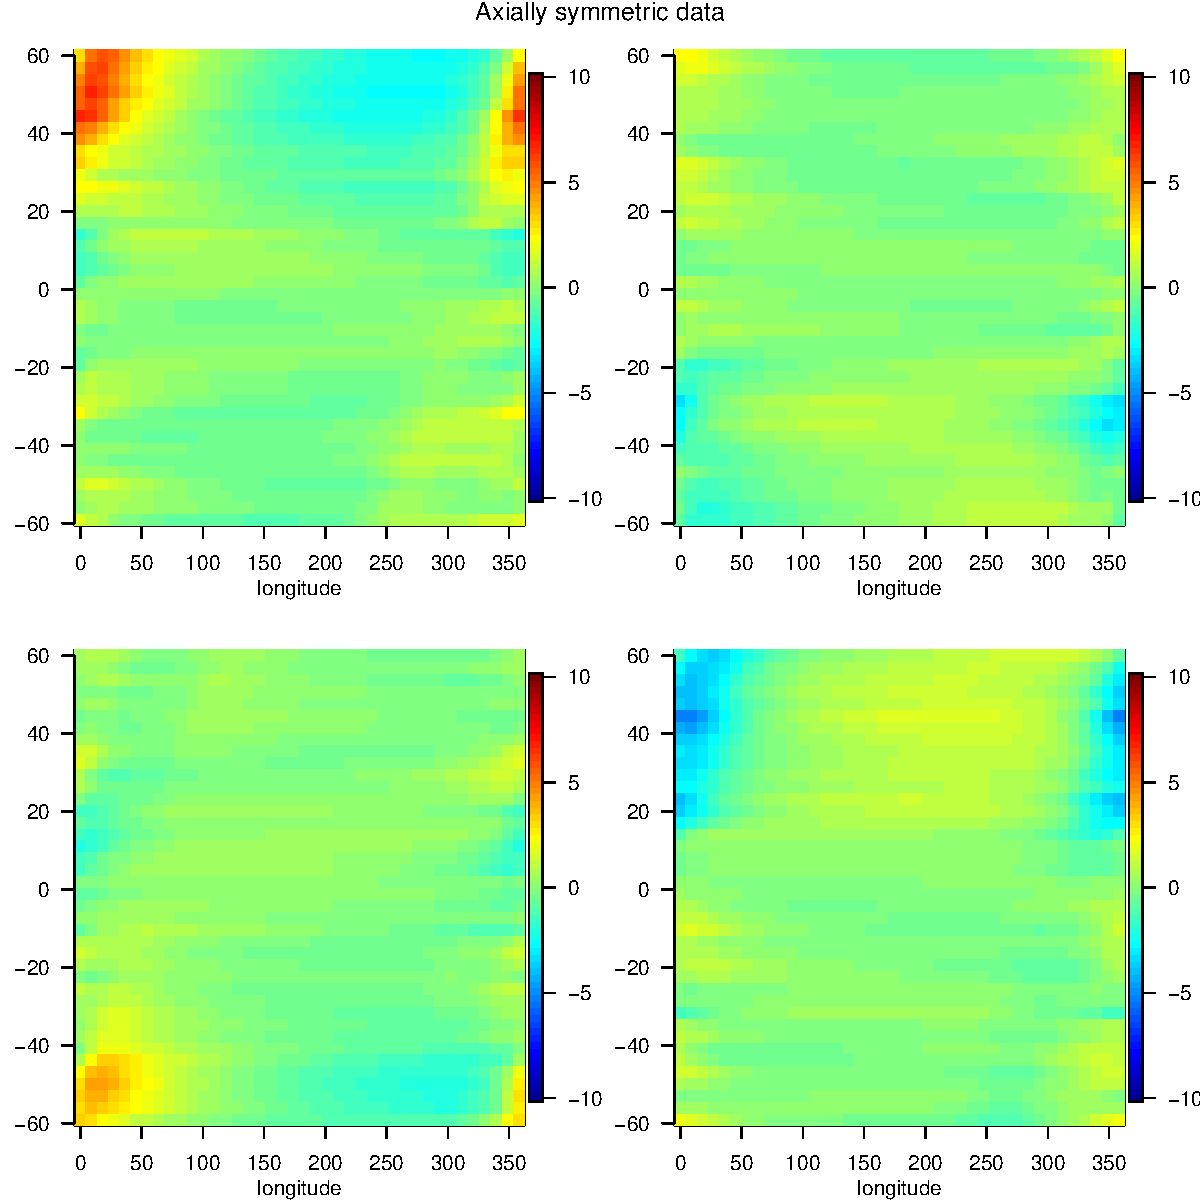
\includegraphics [width=0.9\textwidth ]{graphs/Data_sample_120_model2.pdf}
		\caption{Four consecutive axially symmetric data snapshots based on model 2, grid resolution $2^0\times 1^0$ (data scale -10 and 10).}
	\end{center}
\end{figure}

The above snapshots are some what compliance with geo-spatial data (MSU and TOMS), clearly there is a spatial trend within each latitude but not within longitudes. We observed some inconsistencies (strong spots) closer to the boundary points of longitudes ($\lambda \rightarrow 0,\lambda \rightarrow 2\pi$) and we have ignored the tilt (approximately $23^0$) of Earth axis, both of these are left out as future studies. The figure \ref{grid_plot_model2_sim2} refers to the second snapshot (top right) of the generated data and it is clearly evident that trends are within latitudes.     

\begin{figure}[H]
	\label{grid_plot_model2_sim2}
	\begin{center}
		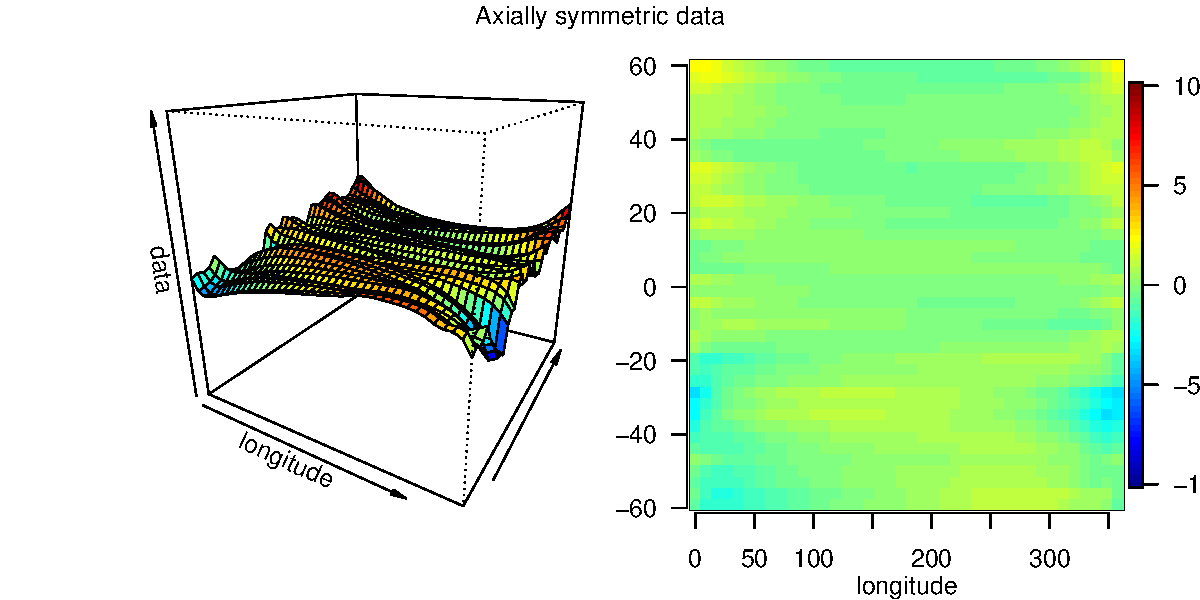
\includegraphics [width=0.9\textwidth ]{graphs/Data_sample_120_model2_density.pdf}
		\caption{One snapshot of the axially symmetric data generated based on model 2, grid resolution $2^0\times 1^0$ (data scale -10 and 10)Data distribution over the grid.}
	\end{center}
\end{figure}

%-------------------------------------% 
\subsection{Comparison of the proposed models with MOM estimates}
%-------------------------------------%

We consider two latitudes with larger latitude difference in order to capture the largest possible errors $70^0S$ and $60^0N$ ($\phi = 10, 150$) with 100 longitudes and compared the MOM estimators.

\begin{figure}[H]
	\begin{subfigure}{.5\textwidth}
		\centering
		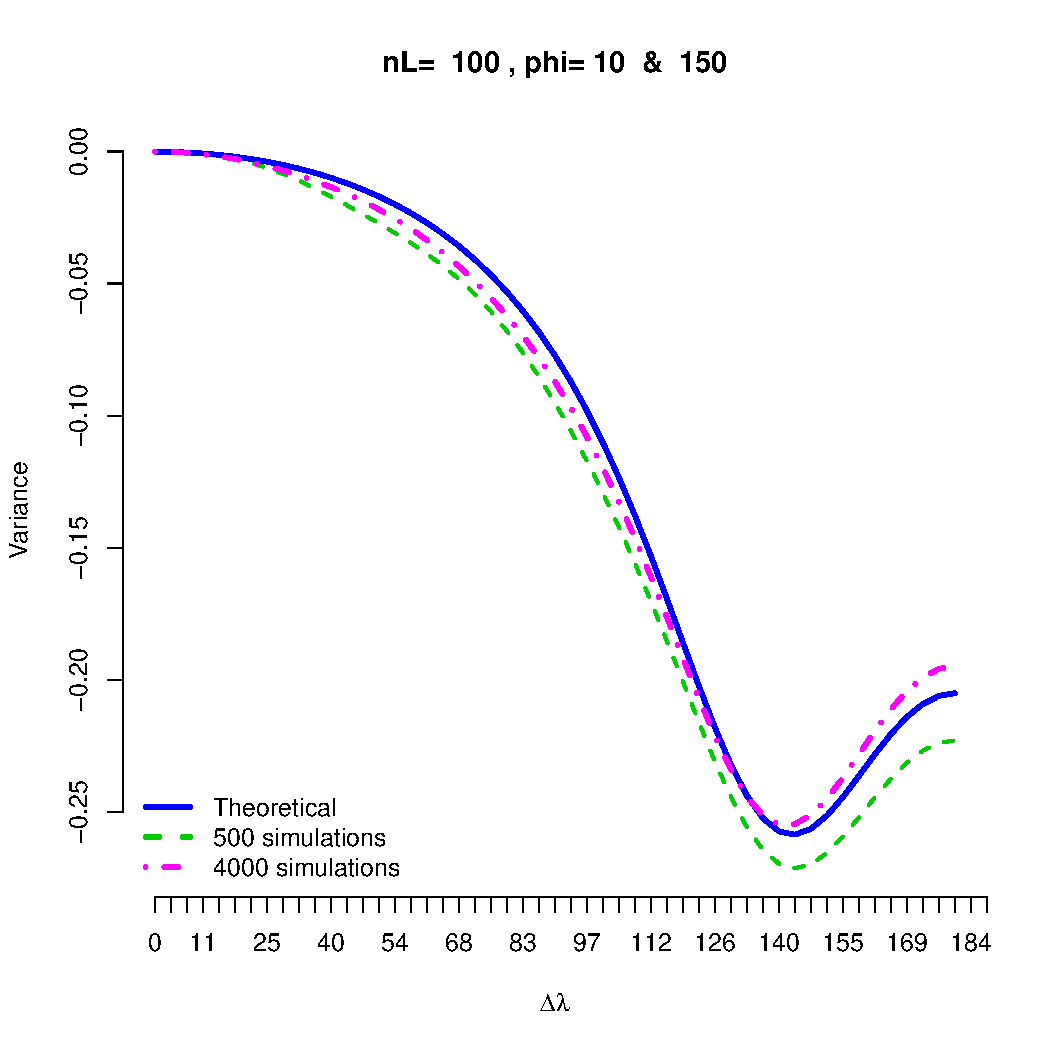
\includegraphics[width=1\linewidth]{graphs/results_variogram_model1}
		\caption{parameter set 1}
		\label{fig:sfig1}
	\end{subfigure}
	\begin{subfigure}{.5\textwidth}
		\centering
		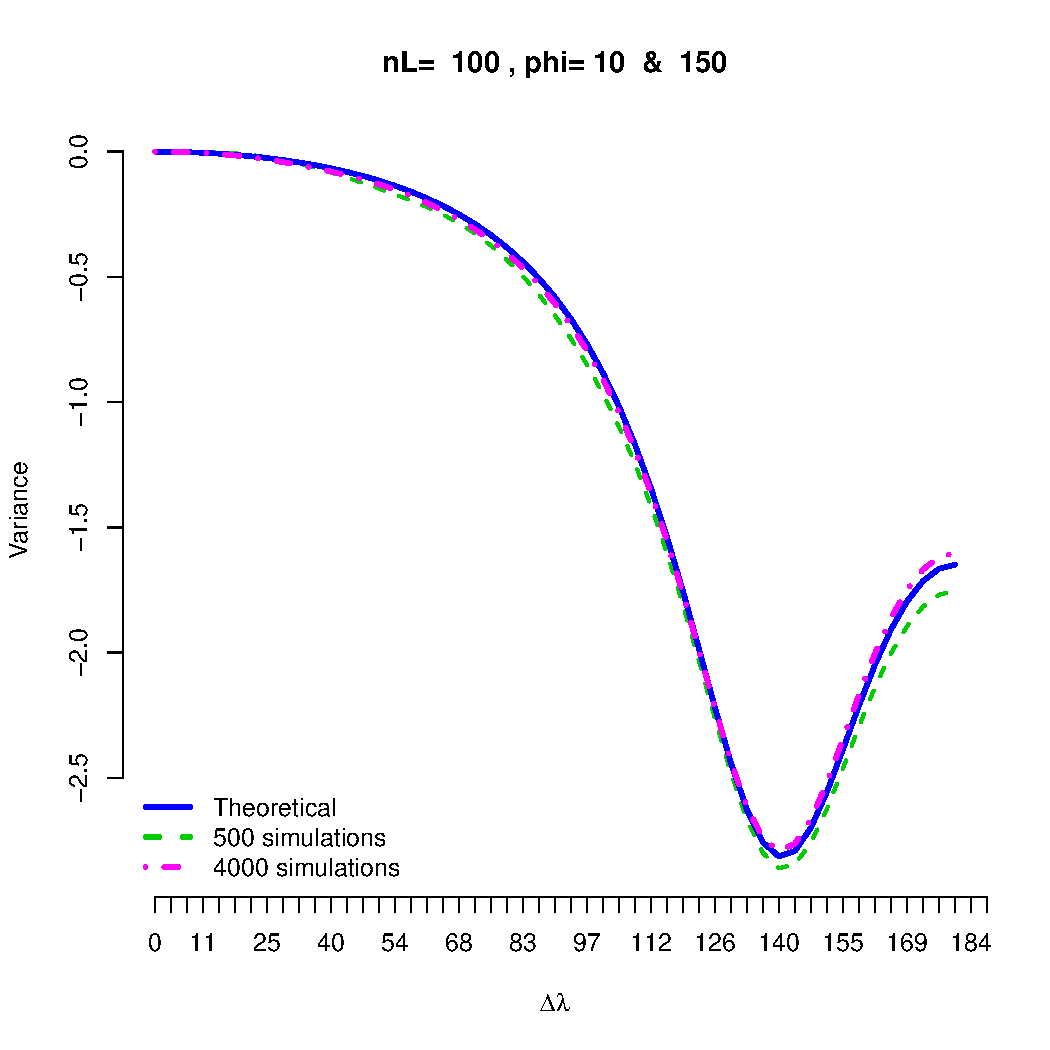
\includegraphics[width=1\linewidth]{graphs/results_variogram_model1_2}
		\caption{parameter set 2}
		\label{fig:sfig2}
	\end{subfigure}
	\caption[Cross variogram estimator comparison]{Cross variogram estimator comparison for covariance model1 }
	\label{compare_varigram_sim}
\end{figure}

The cross variogram estimator (\ref{cross_variogram}) is unbiased and in case of circle we showed that the variogram estimator is inconsistent and we expect a similar result in the case of sphere (the proof is left out as future work). Since model 1 is a non zero mean process we use the cross variogram estimator () to compare the generated data. We used two different sets of parameters to compare the cross variogram for model 1, set 1 $C_1 = 1, C_2 = 1, a = 1, u = 1$ and $p=0.5$ and set 2 $C_1 = C_2 = 2, a = =3, u = 1$ and $p=0.6$. The rate of convergence (\blue{should we talk about any theoretical properties of convergence since we don't have a proof for consistency}) is very slow as one can see that when number of simulations were increased from 500 to 4000 the cross variogram estimator is much closer to its theoretical value. However, the cross variogram estimator for model 2 and 3 converges much faster compared to model 1.  

%-------------------------------------% 
\subsubsection{Results for longitudinally reversible processes}
%-------------------------------------%

The parameter $u = 0$ yields a longitudinally reversible processes on a sphere (see Figure \ref{fig_parameter_comp} 1(d) ) regardless of the model. Now the cross variogram estimator converges ({\em a.s.}) to its theoretical value much faster (< 500 simulations).          

\begin{figure}[H]
	\centering
	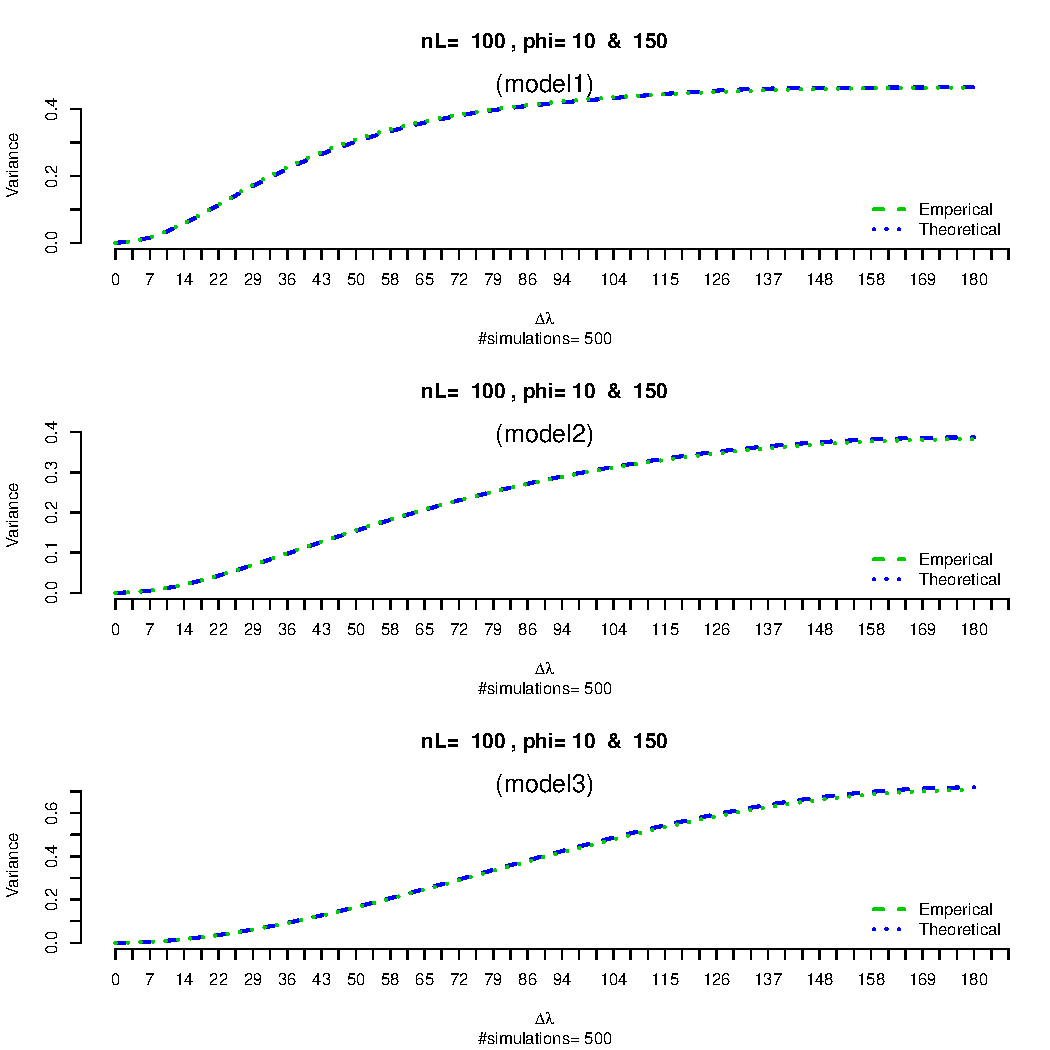
\includegraphics [width=0.9\textwidth ]{graphs/results_variogram_comparison}
	% width=12cm,height=12cm
	\caption[Variogram comparison]{Cross variogram estimator comparison over model 1, model 2, model 3 when $u=0$ }
\end{figure}

Next, we compared the cross covariance estimator on zero mean processes (model 2, model 3) on a sphere. In order to compare the cross covariance we used two pairs of latitudes $20^0S$ with $10^0S$ ($\phi = 70, 80$) and $30^0S$ with $40^0N$ ($\phi = 60, 120$). In a zero mean process, the rate of convergence depends on the distance between the latitudes.    

% \begin{figure}[H]
% \begin{center}
% 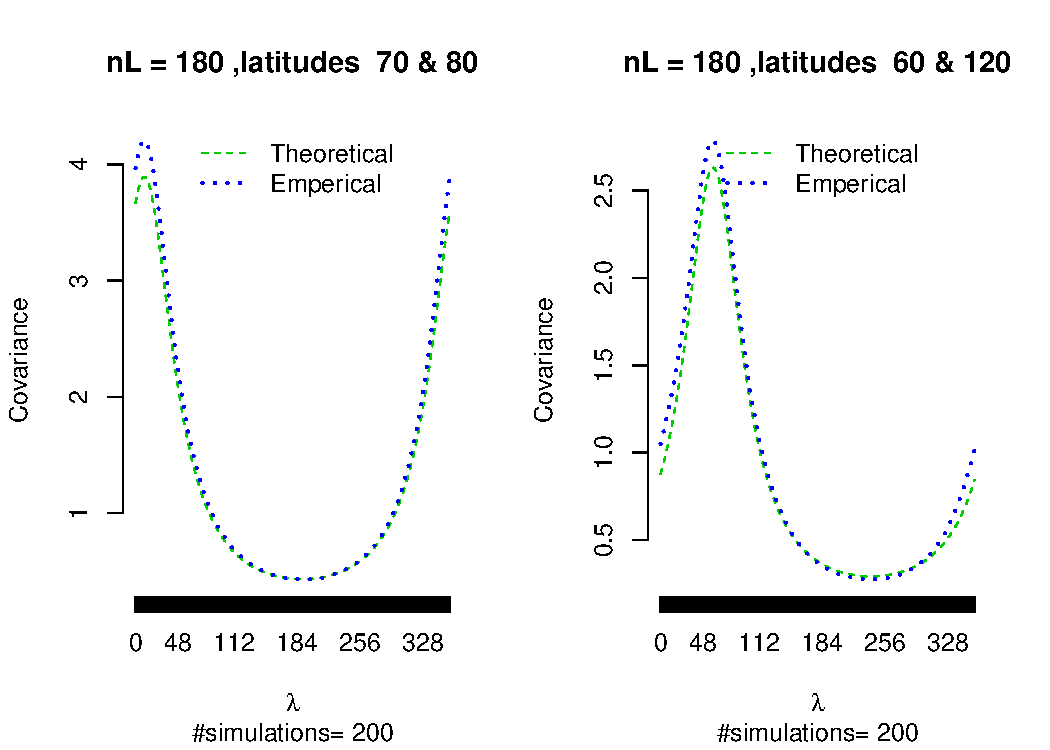
\includegraphics [width=0.75\textwidth ]{graphs/Model1.pdf}
% \caption{Cross covariance comparison of model1}
% \end{center}
% \end{figure}



\begin{figure}[H]
	\begin{center}
		\includegraphics [width=0.75\textwidth ]{graphs/Model2.pdf}
		%\includegraphics [width=6in, height=3in]{Model2.pdf}
		\caption{Cross covariance comparison of model 2}
	\end{center}
\end{figure}


\begin{figure}[H]
	\begin{center}
		%\includegraphics [scale=.6]{Model3.pdf}
		\includegraphics [width=0.75\textwidth ]{graphs/Model3.pdf}
		\caption{Cross covariance comparison of model 3}
	\end{center}
\end{figure}




%\end{document}

			
